% ------------------------------------------------------------------------------
% TYPO3 CMS 7.0 - What's New - Chapter "Introduction" (Dutch Version)
%
% @author	Michael Schams <schams.net>
% @license	Creative Commons BY-NC-SA 3.0
% @link		http://typo3.org/download/release-notes/whats-new/
% @language	Dutch
% ------------------------------------------------------------------------------
% LTXE-CHAPTER-UID:		2e356b96-2b371a30-940565af-35d5aaf8
% LTXE-CHAPTER-NAME:	Introduction
% ------------------------------------------------------------------------------

\section{Inleiding}
\begin{frame}[fragile]
	\frametitle{Inleiding}

	\begin{center}\huge{Inleiding}\end{center}
	\begin{center}\huge{\color{typo3darkgrey}\textbf{De feiten}}\end{center}

\end{frame}

% ------------------------------------------------------------------------------
% LTXE-SLIDE-START
% LTXE-SLIDE-UID:		66768621-e35a8b65-bc227d15-19215167
% LTXE-SLIDE-ORIGIN:	c0dd5662-b64f5b3d-ea39556c-dca19b07 English
% LTXE-SLIDE-TITLE:		TYPO3 CMS 7.0 - The Facts
% ------------------------------------------------------------------------------

\begin{frame}[fragile]
	\frametitle{Inleiding}
	\framesubtitle{TYPO3 CMS 7.0 - De feiten}

	\begin{itemize}
		\item Publicatiedatum: 2 december 2014
		\item Publicatietype: "Sprint Release"
		\item Visie: Omarm, Innoveer, Verspreid
		\item Primaire focus: backend makeover
	\end{itemize}

	\begin{figure}
		
\includegraphics[width=0.95\linewidth]{typo3-seven-zero-banner.png}
	\end{figure}

\end{frame}

% ------------------------------------------------------------------------------
% LTXE-SLIDE-START
% LTXE-SLIDE-UID:		f0361250-30481d9f-4c4fb64e-a2062f00
% LTXE-SLIDE-ORIGIN:	f0c768bc-7a7f5fff-20ca5059-23f8e843 English
% LTXE-SLIDE-TITLE:		System Requirements
% ------------------------------------------------------------------------------

\begin{frame}[fragile]
	\frametitle{Inleiding}
	\framesubtitle{Systeemeisen	}

	\begin{itemize}
		\item PHP*:\tabto{2.2cm}v5.5.0 - v5.6.x
		\item MySQL:\tabto{2.2cm}v5.5.x - v5.6.x (geen strict mode)
		\item Schijfruimte:\tabto{2.2cm}min 200 MB
		\item PHP-instellingen:

			\begin{itemize}
				\item memory\_limit >= 128M
				\item max\_execution\_time >= 240s
				\item compilatie optie \texttt{-}\texttt{-disable-ipv6} \underline{niet} gebruiken
			\end{itemize}

		\item Backend vereist IE >= 9 of een andere moderne browser

	\end{itemize}

	\vspace{1cm}
	*) Meer details: \href{http://typo3.org/news/article/php-minimum-requirements-for-typo3-cms-7/}{PHP Minimum Requirements for TYPO3 CMS 7}

\end{frame}

% ------------------------------------------------------------------------------
% LTXE-SLIDE-START
% LTXE-SLIDE-UID:		acf028f6-696b3074-d7a49a0b-169dccc0
% LTXE-SLIDE-ORIGIN:	e6dd8a1b-2b60f76b-adc1d788-f77036d9 English
% LTXE-SLIDE-TITLE:		Development And Release Timeline
% ------------------------------------------------------------------------------

\begin{frame}[fragile]
	\frametitle{Inleiding}
	\framesubtitle{Ontwikkelings- en publicatietijdlijn}

	\begin{figure}
		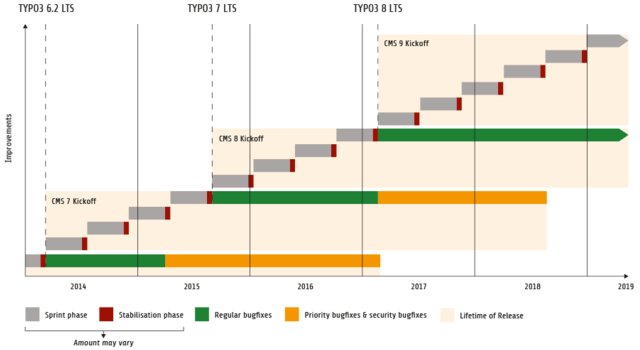
\includegraphics[width=0.90\linewidth]{Introduction/ReleaseAgenda.png}
	\end{figure}

\end{frame}

% ------------------------------------------------------------------------------
% LTXE-SLIDE-START
% LTXE-SLIDE-UID:		0dac057e-20e0c72d-aa068ea1-16c95df5
% LTXE-SLIDE-ORIGIN:	a99cfec1-0a35c0fb-e552ac34-e4e407f8 English
% LTXE-SLIDE-TITLE:		TYPO3 CMS Roadmap
% ------------------------------------------------------------------------------
% https://typo3.org/typo3-cms/roadmap/

\begin{frame}[fragile]
	\frametitle{Inleiding}
	\framesubtitle{TYPO3 CMS Roadmap}

	Geschatte publicatiedatum en primaire focus:

	\begin{itemize}
		\item
			\begingroup
				\color{typo3orange}
					v7.0 \textrightarrow\tabto{1.3cm}02 dec 2014\tabto{3.4cm}Backend makeover deel 1
			\endgroup

		\item v7.1 \textrightarrow\tabto{1.3cm}17 feb 2015\tabto{3.4cm}Core Cleanup \& Streamlining
		\item v7.2 \textrightarrow\tabto{1.3cm}10 mar 2015\tabto{3.4cm}Frontend
		\item v7.3 \textrightarrow\tabto{1.3cm}21 apr 2015\tabto{3.4cm}Composer Ecosysteem
		\item v7.4 \textrightarrow\tabto{1.3cm}09 jun 2015\tabto{3.4cm}Backend makeover deel 2
		\item v7.5 \textrightarrow\tabto{1.3cm}28 jul 2015\tabto{3.4cm}\textit{(nog onbekend...)}
		\item v7.6 \textrightarrow\tabto{1.3cm}13 oct 2015\tabto{3.4cm}pre-LTS gekte
		\item v7.7 \textrightarrow\tabto{1.3cm}xx xxx 2015\tabto{3.4cm}\textbf{TYPO3 CMS 7 LTS} (Long Term Release)
	\end{itemize}

	\smaller
		\url{https://typo3.org/typo3-cms/roadmap/}\newline
		\url{http://typo3.org/news/article/embrace-and-innovate-typo3-cms-7/}
	\normalsize

\end{frame}

% ------------------------------------------------------------------------------
% LTXE-SLIDE-START
% LTXE-SLIDE-UID:		b9724628-4ab6b1f9-233c79e6-b5b905c8
% LTXE-SLIDE-ORIGIN:	185b2d64-63cab652-fa469322-8a16b1b7 English
% LTXE-SLIDE-TITLE:		Installation
% LTXE-SLIDE-REFERENCE:	https://forge.typo3.org/issues/62578
% ------------------------------------------------------------------------------

\begin{frame}[fragile]
	\frametitle{Inleiding}
	\framesubtitle{Installatie}

	\begin{itemize}
		\item Officiële installatieprocedure op Linux/Mac OS X\newline
			(DocumentRoot bijvoorbeeld \texttt{/var/www/site/htdocs}):
		\begin{lstlisting}
			$ cd /var/www/site
			$ wget --content-disposition get.typo3.org/7.0
			$ tar xzf typo3_src-7.0.0.tar.gz
			$ cd htdocs
			$ ln -s ../typo3_src-7.0.0 typo3_src
			$ ln -s typo3_src/index.php
			$ ln -s typo3_src/typo3
			$ touch FIRST_INSTALL
		\end{lstlisting}

		\item Symbolische koppelingen op Microsoft Windows:

			\begin{itemize}
				\item Gebruik \texttt{junction} met Windows XP/2000
				\item Gebruik \texttt{mklink} met Windows Vista en Windows 7
			\end{itemize}

	\end{itemize}
\end{frame}

% ------------------------------------------------------------------------------
% LTXE-SLIDE-START
% LTXE-SLIDE-UID:		e0067947-dde75a6e-b7ab34d2-b332d1d0
% LTXE-SLIDE-ORIGIN:	d884c8cf-25261e85-a2a26fcd-8a64a9cb English
% LTXE-SLIDE-TITLE:		Upgrade to TYPO3 CMS 7
% LTXE-SLIDE-REFERENCE:	https://forge.typo3.org/issues/62578
% ------------------------------------------------------------------------------

\begin{frame}[fragile]
	\frametitle{Inleiding}
	\framesubtitle{Upgrade naar TYPO3 CMS 7.x}

	\begin{itemize}
		\item Upgrades alleen mogelijk van TYPO3 CMS 6.2 LTS
		\item TYPO3 CMS < 6.2 moet eerst worden geüpgrade naar TYPO3 CMS 6.2 LTS
	\end{itemize}

	\begin{itemize}

		\item Upgrade-instructies:\newline
			\smaller\url{http://wiki.typo3.org/Upgrade#Upgrading_to_7.0}\normalsize
		\item Officiële TYPO3-handleiding "TYPO3 Installation and Upgrading":
			\smaller\url{http://docs.typo3.org/typo3cms/InstallationGuide}\normalsize
		\item Algemene aanpak:
			\begin{itemize}
				\item Controleer minimale systeemeisen (PHP, MySQL, etc.)
				\item Inspecteer \textbf{deprecation\_*.log} in oude TYPO3-installatie
				\item Werk alle extensies bij naar de nieuwste versie
				\item Zet nieuwe bronbestanden neer en start\newline
					Installatie-module \textrightarrow Upgrade Wizard
				\item Check startmodule voor backend gebruikers (optioneel)
			\end{itemize}
	\end{itemize}

\end{frame}

% ------------------------------------------------------------------------------
